\section{1174083 - Bakti Qilan Mufid}
Chapter 2 - Membangun model prediksi
\subsection{Teori}
\subsubsection{Jelaskan Apa Itu Binary Classification dilengkapi ilustrasi gambar sendiri.}
\hfill\\
\begin{figure}[H]
    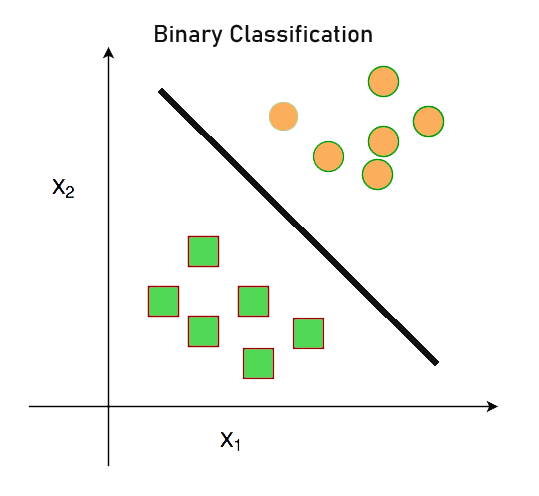
\includegraphics[width=12cm]{figures/1174083/figures2/1.png}
    \centering
    \caption{gambaran binary classification}
\end{figure}

Klasifikasi biner atau binomial adalah tugas mengklasifikasikan elemen-elemen dari himpunan yang diberikan ke dalam dua kelompok (memprediksi kelompok mana yang masing-masing dimiliki) berdasarkan aturan klasifikasi. Konteks yang membutuhkan keputusan apakah suatu item memiliki sifat kualitatif atau tidak, beberapa karakteristik tertentu, atau beberapa klasifikasi biner khas meliputi:
\begin{itemize}
	\item Tes medis untuk menentukan apakah pasien memiliki penyakit tertentu atau tidak - properti klasifikasi adalah keberadaan penyakit.
	\item Metode uji "lulus atau gagal" atau kontrol kualitas di pabrik, yaitu memutuskan apakah suatu spesifikasi telah atau belum terpenuhi - klasifikasi Go/no go.
	\item Pengambilan informasi, yaitu memutuskan apakah suatu halaman atau artikel harus ada dalam hasil pencarian atau tidak - properti klasifikasi adalah relevansi artikel.
\end{itemize}

\subsubsection{Jelaskan Apa itu supervised learning , unsupervised learning dan clusterring dengan ilustrasi gambar sendiri.}
\begin{enumerate}
\item supervised learning
\hfill\\
Supervised learning merupakan suatu pembelajaran yang terawasi dimana jika output yang diharapkan telah diketahui sebelumnya. Biasanya pembelajaran ini dilakukan dengan menggunakan data yang telah ada. Dan Supervised Learning dalam bahasa indonesia adalah pembelajaran yang ada supervisornya. Maksud disini ada supervisornya adalah label di tiap data nya. Label maksudnya adalah tag dari data yang ditambahkan dalam machine learning model. Contohnya gambar kucing di tag “kucing” di tiap masing masing image kucing dan gambar anjing di tag “anjing” di tiap masing gambar anjing.
\begin{figure}[H]
    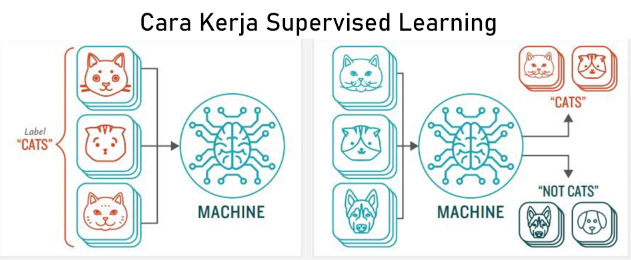
\includegraphics[width=12cm]{figures/1174083/figures2/2.png}
    \centering
    \caption{gambaran cara kerja supervised}
\end{figure}

\item unspervised learning
\hfill\\
Unsupervised learning memiliki keunggulan daari supervised learning. Jika supervised learning memiliki label sebagai dasar prediksi baik serta membuat clasification dan regression algorithm yang memungkinkan. Tetapi dalam realitanya, data real itu banyak yang tidak memiliki label. Unsupervised learning menggunakan ke samaan dari attribut attribut yang dimiliki. Jika attribut dan sifat sifat dari data data feature yang diekstrak memiliki kemirip miripan, maka akan dikelompok kelompokan (clustering). Sehingga hal ini akan menimbulkan kelompok kelompok (cluster). Jumlah cluster bisa unlimited. Dari kelompok kelompok itu model melabelkan, dan jika data baru mau di prediksi, maka akan dicocok kan dengan kelompok yang mirip mirip featurenya.
\begin{figure}[H]
    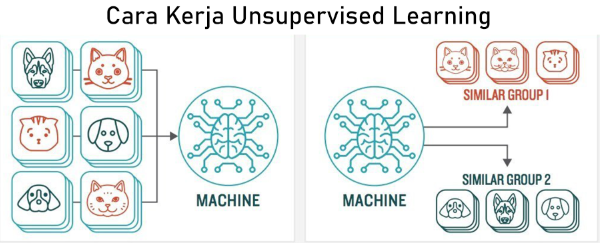
\includegraphics[width=12cm]{figures/1174083/figures2/3.png}
    \centering
    \caption{gambaran cara kerja unsupervised}
\end{figure}

\item Clustering 
\hfill\\
Clustering adalah sebuah metode untuk membedakan data - data menjadi kumpulan dari group yang isinya merupakan data yang serupa setiap grupnya. Basisnya dapat berupa kesamaan atau perbedaan dari setiap grup tersebut.
\begin{figure}[H]
    
\includegraphics[width=12cm]{figures/1174083/figures2/4.png}
    \centering
    \caption{gambaran clustering}
\end{figure}
\end{enumerate}
\subsubsection{Jelaskan apa itu evaluasi dan akurasi dan disertai ilustrasi contoh dengan gambar sendiri}
\hfill\\
Evaluasi adalah tentang bagaimana kita dapat mengevaluasi seberapa baik model bekerja dengan mengukur akurasinya. Dan akurasi akan didefinisikan sebagai persentase kasus yang diklasifikasikan dengan benar. Kita dapat menganalisis kesalahan yang dibuat oleh model,atau tingkat kebingungannya,menggunakan matriks kebingungan(\textit{confusion matrix}) . Matriks kebingungan mengacu pada kebingungan dalam model,tetapi matriks kebingungan ini bisa menjadi sedikit sulit untuk dipahami ketika mereka menjadi sangat besar.
\begin{figure}[H]
    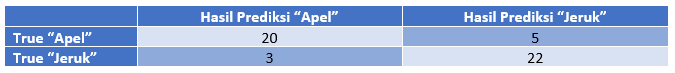
\includegraphics[width=12cm]{figures/1174083/figures2/5.png}
    \centering
    \caption{contoh confusion matrix}
\end{figure}

\subsubsection{Jelaskan bagaimana cara membuat Confusion Matrix, Buat confusion matrix sendiri.}
\hfill\\
Confusion Matrix merupakan metode untuk menghitung akurasi pada data mining atau Sistem Pendukung Keputusan. Untuk menggunakan Confusion Matrix, ada 4 istilah sebagai hasil proses dari klasifikasi. Diantaranya adalah :
\begin{itemize}
    \item True Positive : Data positif yang terdeteksi memiliki hasil benar
    \item False Positive : Data Positif yang terdeteksi memiliki hasil salah
    \item True Negative : Data negatif yang terdeteksi memiliki hasil benar
    \item False Negative : Data negatif yang terdeteksi memiliki hasil salah
\end{itemize}
\begin{figure}[H]
    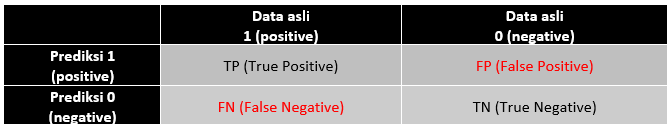
\includegraphics[width=12cm]{figures/1174083/figures2/6.png}
    \centering
    \caption{contoh confusion matrix}
\end{figure}	

\subsubsection{Jelaskan bagaimana K-fold cross validation bekerja dengan gambar ilustrasi contoh buatan sendiri.}
\hfill\\
Cara kerja k-fold validation:
\begin{itemize}
	\item Total instance dibagi menjadi N bagian.
	\item Fold yang pertama adalah bagian pertama menjadi data uji (testing data) dan sisanya menjadi training data.
	\item Lalu hitung akurasi berdasarkan porsi data tersebut dengan menggunakan persamaan.
	\item Fold yang kedua adalah bagian kedua, yang menjadi data uji(testing data)dan sisanya training  data.
	\item Kemudian hitung akurasi berdasarkan porsi data tersebut.
	\item Dan seterusnya hingga habis mencapai fold ke-K.
	\item Terakhir hitung rata-rata akurasi K buah.
\end{itemize}
\begin{figure}[H]
    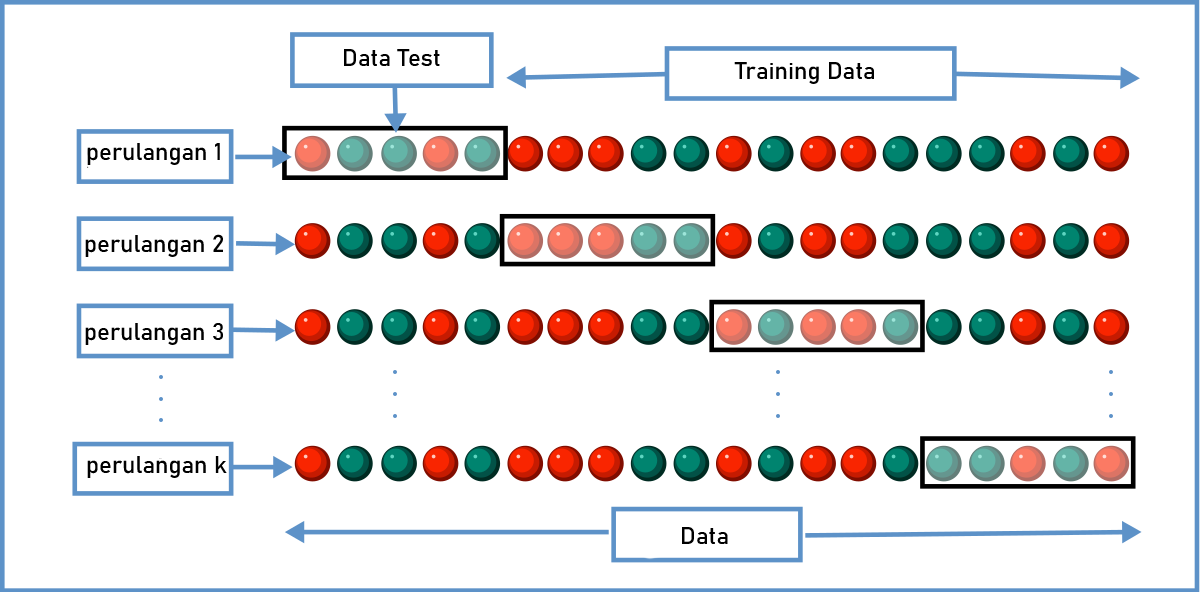
\includegraphics[width=8cm]{figures/1174083/figures2/7.png}
    \centering
    \caption{contoh K-Fold Validation}
\end{figure}

\subsubsection{Jelaskan Apa itu decision tree dengan gambar ilustrasi contoh buatan sendiri.}
\hfill\\
Decision Tree merupakan sebuah struktur yang menentukan keputusan dan setiap konsekuensinya. Hasil dari setiap struktur biasanya menggunakan jawaban (True dan False) atau cabang lain yang akan menjadi pohon selanjutnya. Setiap keputusan diantaranya akan membandingkan kondisi yang diberikan kepada struktur untuk dibandingkan kondisi apa saja yang sudah didapat pada sistem tersebut.
\begin{figure}[H]
    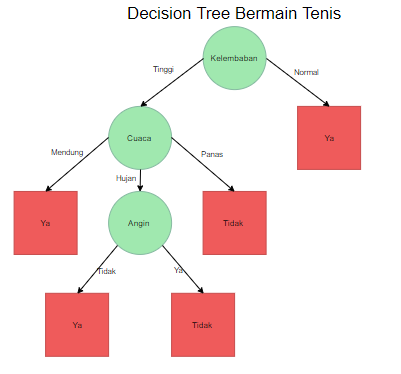
\includegraphics[width=8cm]{figures/1174083/figures2/8.png}
    \centering
    \caption{Decision Tree bermain Tenis}
\end{figure}


\subsubsection{jelaskan apa itu information gain dan entropi dengan gambar ilustrasi buatan sendiri.}
\hfill\\
\begin{enumerate}
	\item information Gain
	\hfill\\
	Information Gain merupakan total data yang didapat dari data - data acak yang data tersebut akan digunakan untuk analisis data lainnya. Information Gain ini digunakan pada decision tree sebagai label setiap aksi - aksi yang perlu dinilai validasinya. 
\begin{figure}[H]
    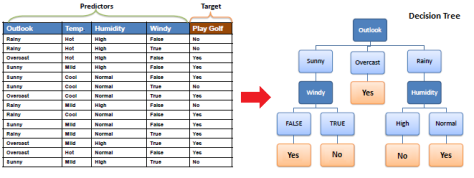
\includegraphics[width=12cm]{figures/1174083/figures2/9.png}
    \centering
    \caption{information gain}
\end{figure}

	\item Entropi
	\hfill\\
	Entropi merupakan pengukuran sebuah data dan validnya data tersebut untuk dapat digunakan sebagai informasi yang akan dimasukkan ke Information Gain. Entropi menilai sebuah obyek berdasarkan kebutuhan di dunia nyata dan pengaruh pada sistem yang akan digunakan.
\begin{figure}[H]
    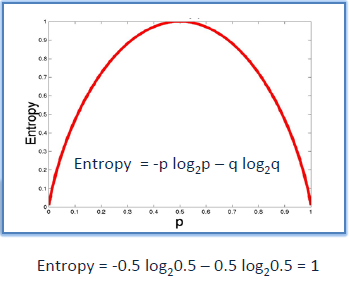
\includegraphics[width=8cm]{figures/1174083/figures2/10.png}
    \centering
    \caption{penggambaran entropi}
\end{figure}
\end{enumerate}



\subsection{Praktek}
Tugas anda adalah, dataset ganti menggunakan student-mat.csv dan mengganti semua nama variabel dari kode di bawah ini dengan nama-nama makanan (NPM mod 3=0), kota (NPM mod 3=1), buah (NPM mod 3=2),
\lstinputlisting[firstline=9, lastline=10]{src/1174083/src2/Student performance.py} 

\subsubsection{Praktek No. 1}
\hfill\\
\lstinputlisting[firstline=13, lastline=16]{src/1174083/src2/Student performance.py}
mengimport library pandas lalu menamainya dengan pd. membuat variable mochi yang didalamnya terdefinisikan perintah untuk membaca file csv. dan len(mochi) untuk mengembalikan panjang jumlah anggota yang dimiliki variabel mochi. 

\begin{figure}[H]
    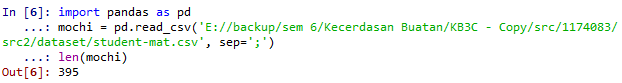
\includegraphics[width=8cm]{figures/1174083/figures2/p1.png}
    \centering
    \caption{Loading Dataset}
\end{figure}

\subsubsection{Praktek No. 2}
\hfill\\
\lstinputlisting[firstline=19, lastline=22]{src/1174083/src2/Student performance.py}
pada bagian ini mendeklarasikan pass/fail nya data berdasarkan G1+G2+G3. Dengan ketentuan nilai passnya yaitu lebih besar/sama dengan 30. kemudian pada variabel mochi dideklarasikan jika baris dengan G1+G2+G3 ditambahkan,dan hasilnya lebih besar/sama dengan 35 maka axisnya 1. ketika dijalankan hasilnya seperti berikut

\begin{figure}[H]
    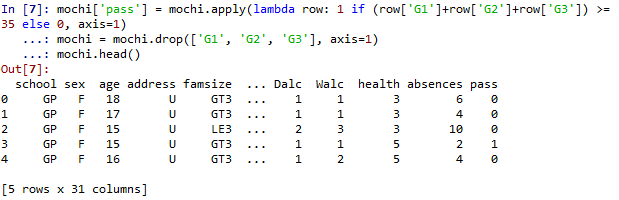
\includegraphics[width=8cm]{figures/1174083/figures2/p2.png}
    \centering
    \caption{Generate Binary Label}
\end{figure}

\subsubsection{Praktek No. 3}
\hfill\\
\lstinputlisting[firstline=25, lastline=29]{src/1174083/src2/Student performance.py}
One-hot encoding adalah proses di mana variabel kategorikal dikonversi menjadi bentuk yang dapat disediakan untuk algoritma ML agar melakukan pekerjaan yang lebih baik dalam prediksi. Karena kita memuat data menggunakan pandas, disini digunakan fungsi panda pdgetdummies untuk jenis kelamin , sekolah, alamat dll. Metode head ini digunakan untuk mengembalikan baris n atas 5 secara default dari frame atau seri data. hasilnya seperti berikut

\begin{figure}[H]
    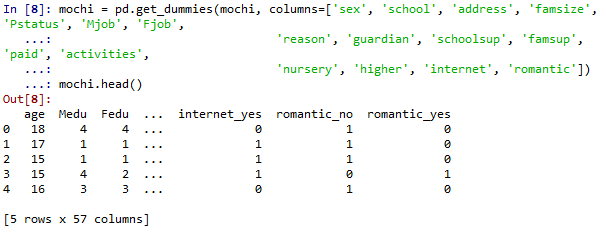
\includegraphics[width=8cm]{figures/1174083/figures2/p3.png}
    \centering
    \caption{One-hot Encoding}
\end{figure}

\subsubsection{Praktek No. 4}
\hfill\\
\lstinputlisting[firstline=32, lastline=50]{src/1174083/src2/Student performance.py}
Sample digunakan untuk mengembalikan(return) sampel secara acak(item) dari objek. Pada bagian tersebut, terdapat train dan test yaing digunakan untuk untuk membagi train, test dan kemudian membagi lagi train ke validasi dan test. Kemudia akan mengimport module numpy sebagai np yang akan digunakan untuk mengembalikan nilai passing dari pelajar dari keseluruhan dataset dengan cara print.

\begin{figure}[H]
    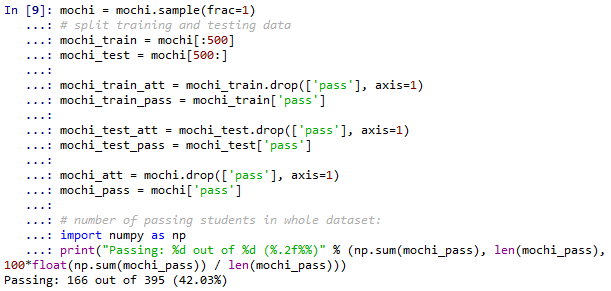
\includegraphics[width=8cm]{figures/1174083/figures2/p4.png}
    \centering
    \caption{Shuffle Rows}
\end{figure}

\subsubsection{Praktek No. 5}
\hfill\\
\lstinputlisting[firstline=53, lastline=57]{src/1174083/src2/Student performance.py}
Dari librari scikit-learn import modul tree. Kemudian definisikan variabel Cilok dengan menggunakan DecisionClassifier.Kemudian pada variabel cilok terdapat Criterion yaitu suatu fungsi untuk mengukur kualitas split,setelah itu agar DecisionTreeClassifier dapat dijalankan gunakan perintah fit. hasilnya seperti dibawah

\begin{figure}[H]
    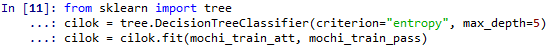
\includegraphics[width=8cm]{figures/1174083/figures2/p5.png}
    \centering
    \caption{Fit Decision tree}
\end{figure}

\subsubsection{Praktek No. 6}
\hfill\\
\lstinputlisting[firstline=62, lastline=68]{src/1174083/src2/Student performance.py}
Graphviz adalah perangkat lunak visualisasi grafik open source. Visualisasi grafik adalah cara mewakili informasi struktural sebagai diagram grafik dan jaringan abstrak. TREEEXPORTGRAPHVIZ merupakan fungsi yang menghasilkan representasi Graphviz dari decision tree,yang kemudian ditulis ke out file. Sehingga akan muncul gambar diagram grafik bercabang.

\begin{figure}[H]
    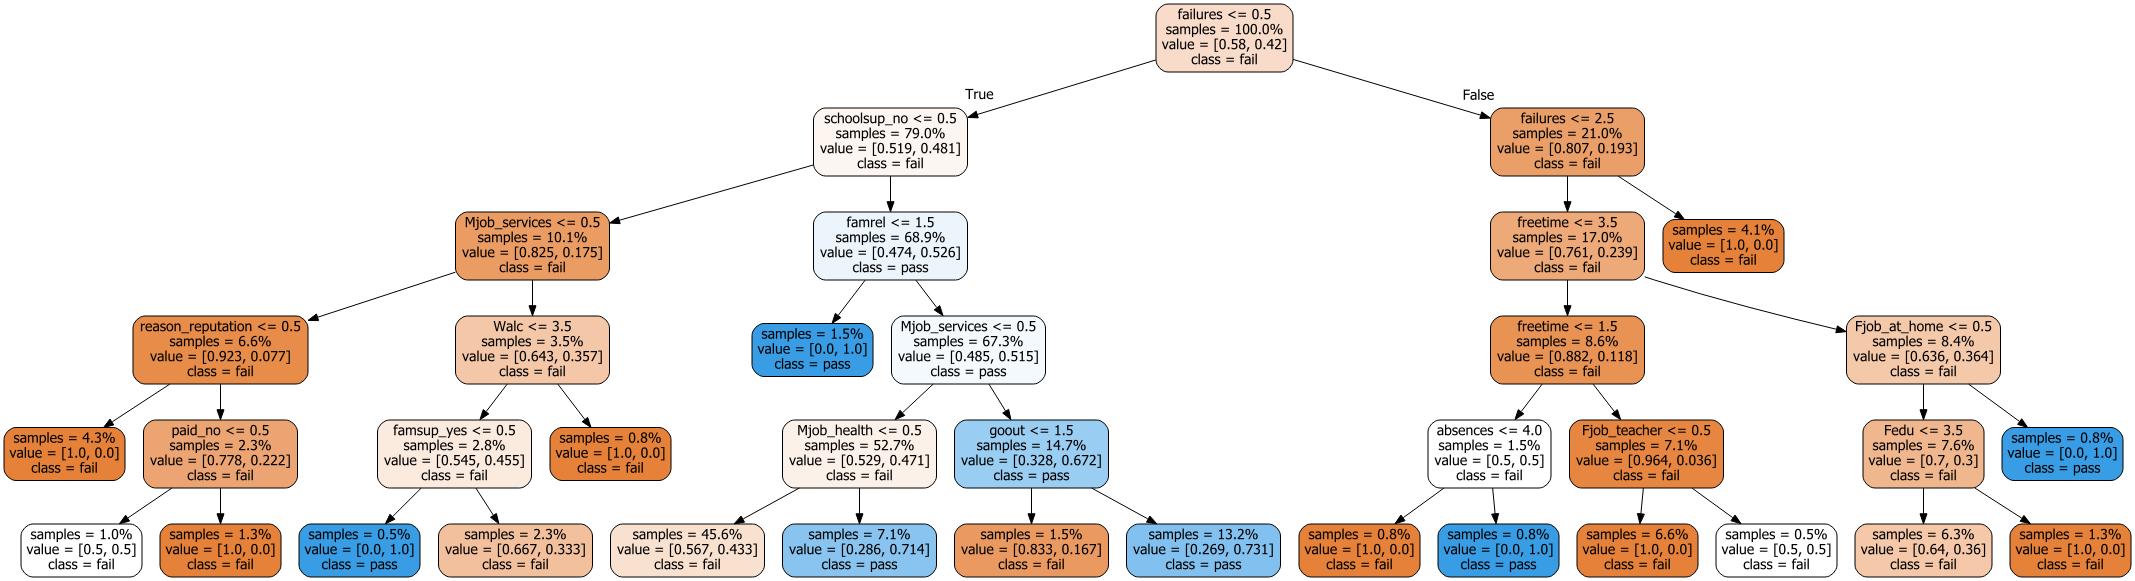
\includegraphics[width=12cm]{figures/1174083/figures2/p6.png}
    \centering
    \caption{Visualize tree}
\end{figure}

\subsubsection{Praktek No. 7}
\hfill\\
\lstinputlisting[firstline=70, lastline=74]{src/1174083/src2/Student performance.py}
TREEEXPORTGRAPHVIZ merupakan fungsi yang menghasilkan representasi  Graphviz dari decision tree,yang kemudian dituliske out file.Disini akan disimpan classifiernya, yang setelahnya akan mengekspor file student performance dan jika salah akan mengembalikan nilai fail.

\begin{figure}[H]
    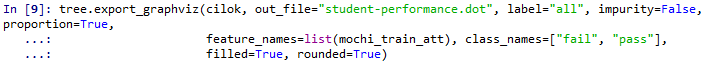
\includegraphics[width=8cm]{figures/1174083/figures2/p7.png}
    \centering
    \caption{menyimpan(save) tree}
\end{figure}

\subsubsection{Praktek No. 8}
\hfill\\
\lstinputlisting[firstline=77, lastline=78]{src/1174083/src2/Student performance.py}
Score juga disebut prediksi,dan merupakan proses yang menghasilkan nilai berdasarkan model pembelajaran mesin yang terlatih, diberi beberapa data input baru. Nilai atau skor yang dibuat dapat mewakili prediksi nilai masa depan, tetapi mereka juga mungkin mewakili kategori atau hasil yang mungkin. Jadi disini cilok akan memprediksi nilai dari mochi\_ test\_ att dan mochi\_ test\_ pass. Hasilnya seperti dibawah ini 

\begin{figure}[H]
    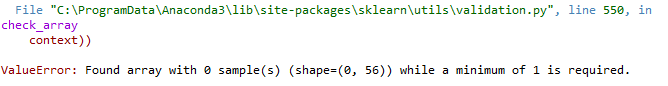
\includegraphics[width=8cm]{figures/1174083/figures2/error3.png}
    \centering
    \caption{Score(masih error)}
\end{figure}

\subsubsection{Praktek No. 9}
\hfill\\
\lstinputlisting[firstline=80, lastline=84]{src/1174083/src2/Student performance.py}
Script ini akan mengevaluasi score dengan validasi silang. Dimana variabel biskuit berisikan cross valscore yang merupakan fungsi pembantu pada estimator dan dataset. Kemudian akan menampilkan score rata rata dan kurang lebih dua standar deviasi yang mencakup 95\% score. dengan menggunakan perintah print hasil yang didapatkan sebagai berikut

\begin{figure}[H]
    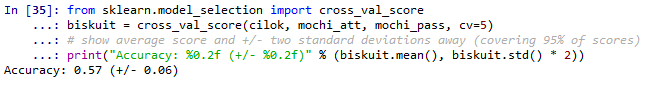
\includegraphics[width=8cm]{figures/1174083/figures2/p9.png}
    \centering
    \caption{Cross Val Score}
\end{figure}

\subsubsection{Praktek No. 10}
\hfill\\
\lstinputlisting[firstline=87, lastline=91]{src/1174083/src2/Student performance.py}
Pada script ini menunjukkan seberapa dalam tree itu. Semakin dalam tree, semakin banyak perpecahan yang dimilikinya dan menangkap lebih banyak informasi tentang data. variabel cilok akan mendefinisikan tree nya yang kemudian variabel biskuit akan mengevaluasi score dengan validasi silang. disini mendefinisikan decision tree dengan kedalaman mulai dari 1 hingga 19 dan merencanakan pelatihan dan menguji skor auc. Jika di run hasilnya seperti berikut

\begin{figure}[H]
    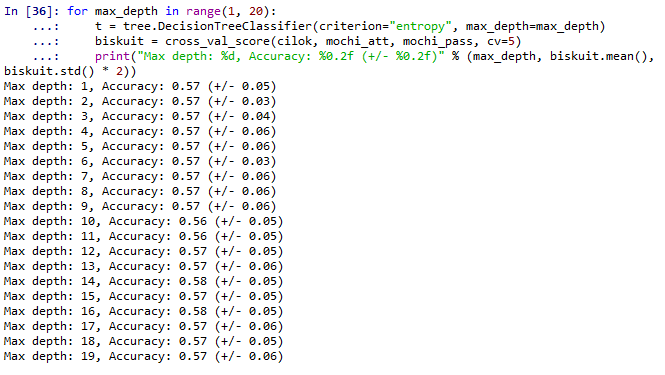
\includegraphics[width=8cm]{figures/1174083/figures2/p10.png}
    \centering
    \caption{Max Depth}
\end{figure}

\subsubsection{Praktek No. 11}
\hfill\\
\lstinputlisting[firstline=93, lastline=103]{src/1174083/src2/Student performance.py}
Depth acc akan membuat array kosong dengan mengembalikan array baru dengan bentuk dan tipe yang diberikan, tanpa menginisialisasi entri. Dengan 19 sebagai bentuk array kosong, 3 sebagai output data-type dan float urutan kolom utama (gaya Fortran) dalam memori. variabel cilok yang akan melakukan split score dan biskuit akan memvalidasi score secara silang. dan pada akhirnya biskuit.std() yaitu menghitung standar deviasi dari data yang diberikan (elemen array) di sepanjang sumbu yang ditentukan (jika ada), hasilnya sebagai berikut

\begin{figure}[H]
    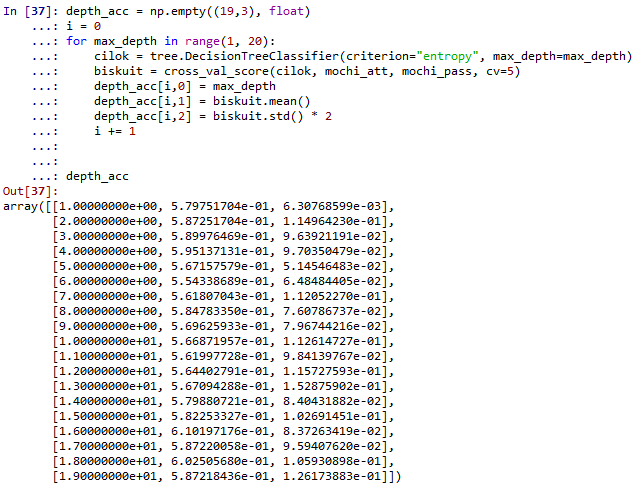
\includegraphics[width=8cm]{figures/1174083/figures2/p11.png}
    \centering
    \caption{Depth in Range}
\end{figure}

\subsubsection{Praktek No. 12}
\hfill\\
\lstinputlisting[firstline=106, lastline=110]{src/1174083/src2/Student performance.py}
Mengimpor librari dari matplotlib yaitu pylot sebagai plt, fig dan puding menggunakan subplots untuk membuat gambar dan satu set subplot. puding.errorbar akan membuat error bar kemudian grafik akan ditampilkan menggunakan show. Grafiknya seperti berikut

\begin{figure}[H]
    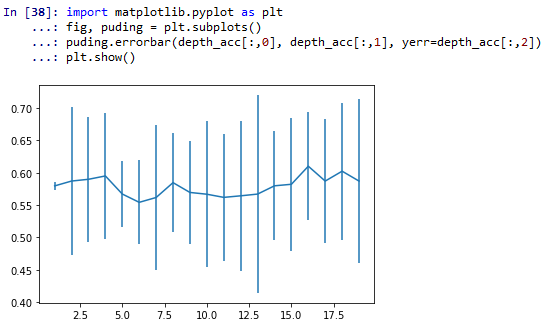
\includegraphics[width=8cm]{figures/1174083/figures2/p12.png}
    \centering
    \caption{Matplotlib}
\end{figure}

\subsection{Penanganan Error}
\subsubsection{Error ke-1}
\hfill\\
\begin{figure}[H]
    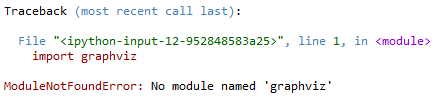
\includegraphics[width=8cm]{figures/1174083/figures2/error1.png}
    \centering
    \caption{No module named graphviz}
\end{figure}
Solusi: 
	\begin{itemize}
	\item buka anaconda navigator $>$ Environment $>$  lalu install graphviz
	\begin{figure}[H]
    	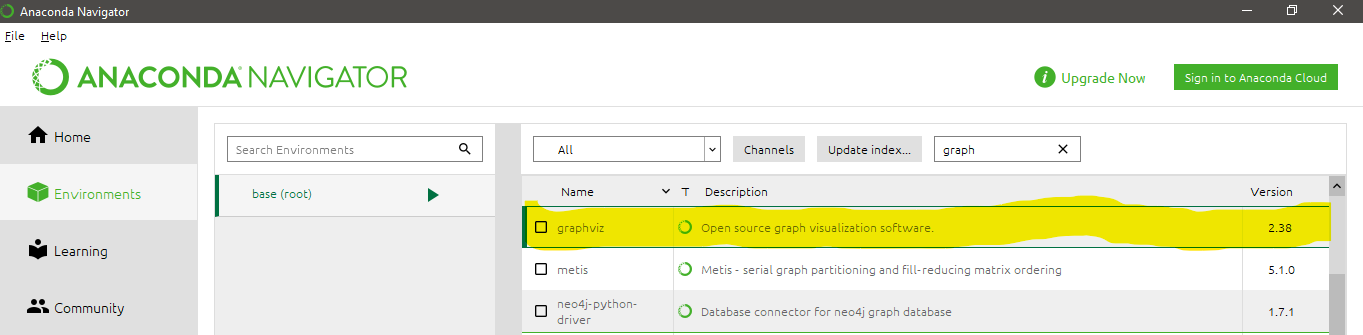
\includegraphics[width=8cm]{figures/1174083/figures2/s1.png}
    	\centering
    	\caption{Solusi dengan anaconda navigator}
	\end{figure}
	\item buka anaconda promt(Run As Admin) $>$ lalu ketikan kode seperti berikut
	\begin{figure}[H]
    	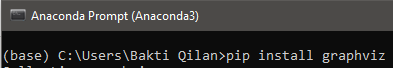
\includegraphics[width=8cm]{figures/1174083/figures2/s1.1.png}
    	\centering
    	\caption{Solusi dengan anaconda promt}
	\end{figure}
	\end{itemize}
	
\subsubsection{Error ke-2}
\hfill\\
\begin{figure}[H]
    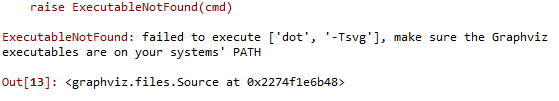
\includegraphics[width=8cm]{figures/1174083/figures2/error2.png}
    \centering
    \caption{graphviz executables}
\end{figure}
Pada gambar diatas kode erornya adalah ExecutableNotFound failed to execute dot Tsvg. Eror ini terjadi karena tidak terdaftarnya environment variable dari Graphviz pada PATH di PC.

Solusi:
menammbahkan kode berikut:
\lstinputlisting[firstline=60, lastline=61]{src/1174083/src2/Student performance.py}

\subsubsection{Error ke-3}
\hfill\\
\begin{figure}[H]
    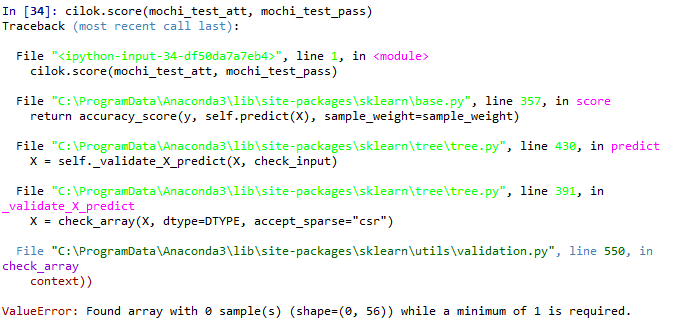
\includegraphics[width=8cm]{figures/1174083/figures2/error4.png}
    \centering
    \caption{Masih belum Paham}
\end{figure}
Solusi:
404 Not Found. Pusing slur!

\subsection{Bukti Tidak Plagiat}
\begin{figure}[H]
	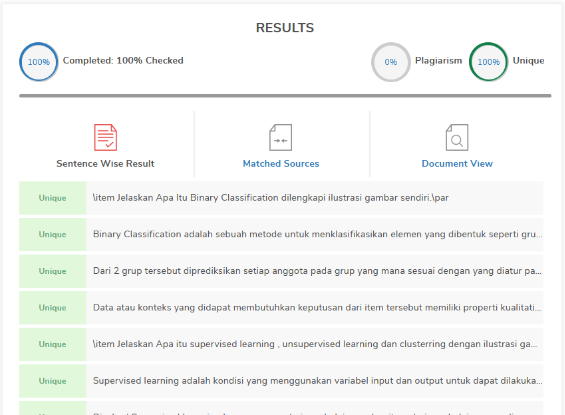
\includegraphics[width=4cm]{figures/1174083/figures2/plagiarism.png}
	\centering
	\caption{plagirism di smallseotools}
\end{figure}

\subsection{Link Video Youtube}
https://youtu.be/19GeYn55DvU
